\begin{figure}[tp]
	\centering
	\subfloat[Table with allowed types for the \mintinline{text}{+} operator]{
		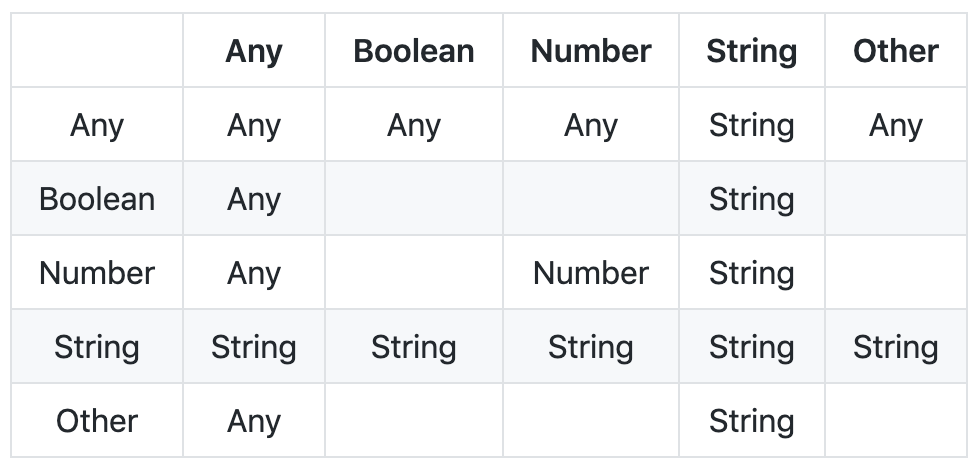
\includegraphics[width=0.6\textwidth]{figures/approach/type-inference/typescript_plus_operator.png}
	}

	\begin{lrbox}{\mintedbox}
		\begin{minipage}{0.7\textwidth}
			\tscode{code/type-inference/constraints/constraints-typescript.ts}
		\end{minipage}
	\end{lrbox}
	\subfloat[Examples of not allowed operations]{\usebox{\mintedbox}}

	\caption[TypeScript definition of the + operator]{\textbf{TypeScript definition of the \mintinline{text}{+} operator} - Rows and columns of the table represent the type of the operands. Values within the table represent the type of the return value. The empty cells specify the invalid operations.}
	\label{fig:type-inference-typescript-definition-plus-operator}
\end{figure}